\newif\ifimagen\imagentrue
\documentclass{book}
\usepackage{hevea}
\usepackage{graphicx}
\usepackage{color}
\def\ccuredversion{1.3.5}
\def\ccuredversion{1.3.5}
\def\ccuredversion{1.3.5}
\def\ccuredversion{1.3.5}
\def\ccuredversion{1.3.5}
\def\ccuredversion{1.3.5}
\newcommand\codecolor{\ifhevea\blue\else\fi}
\renewcommand\c[1]{{\codecolor #1}}
\newcommand\WILD{\t{WILD}}
\newcommand\INDEX{\t{INDEX}}
\newcommand\STRING{\t{STRING}}
\newcommand\ROSTRING{\t{ROSTRING}}
\newcommand\RWSTRING{\t{RWSTRING}}
\newcommand\SEQ{\t{SEQ}}
\newcommand\SEQN{\t{SEQN}}
\newcommand\FSEQ{\t{FSEQ}}
\newcommand\FSEQN{\t{FSEQN}}
\newcommand\SAFE{\t{SAFE}}
\newcommand\RTTI{\t{RTTI}}
\newcommand\SEQR{\t{SEQR}}
\newcommand\FSEQR{\t{FSEQR}}
\newcommand\secref[1]{Section~\ref{sec-#1}}
\newcommand\chref[1]{Chapter~\ref{ch-#1}}
\newcommand\appref[1]{Appendix~\ref{ch-#1}}
\newcommand\browserdoc{\ahrefurl{browser\_help.html}}
\def\code{\begingroup\codecolor\begin{verbatim}}
\def\endcode{\endgroup}
\newcommand\helperdef[3]{
\item \c{#1} \\
\begin{tabular}{ll}
Type inference:\hspace{8mm}& #2\\
At run time:    & #3\\
\end{tabular}
}
\newcommand\helperdefabort[4]{
\item \c{#1} \\
\begin{tabular}{ll}
Type inference: & #2\\
At run time:    & #3\\
Abort condition:\hspace{8mm}& #4\\
\end{tabular}
}
\newcommand\ahreftop[2]{{\ahref{javascript:loadTop('#1')}{#2}}}
\makeatletter
\let\oldmeta\@meta

\def\@meta{%
\oldmeta
\begin{rawhtml}
<base target="main">
<script language="JavaScript">
<!-- Begin
function loadTop(url) {
  parent.location.href= url;
}
// -->
</script>
\end{rawhtml}}
\makeatother

\pagestyle{empty}
\thispagestyle{empty}
\begin{document}
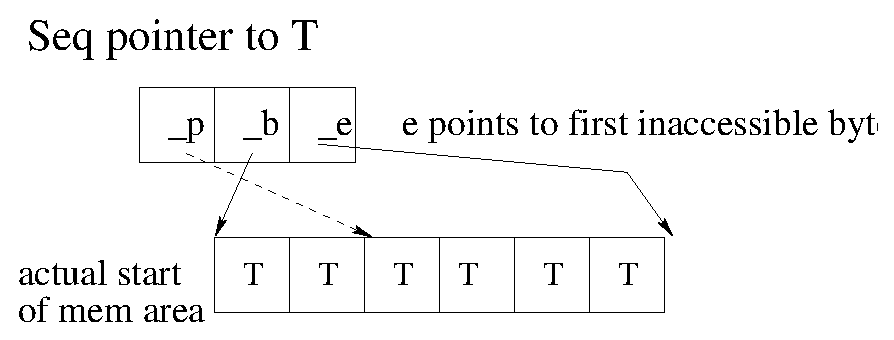
\includegraphics[scale=0.7]{seq.eps}
\clearpage% page: 0
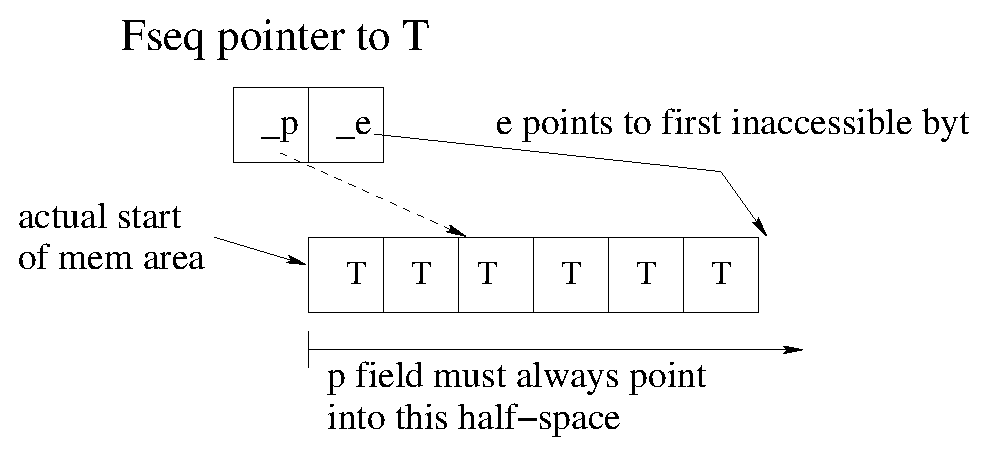
\includegraphics[scale=0.7]{fseq.eps}
\clearpage% page: 1
\includegraphics[scale=0.7]{wild.eps}
\clearpage% page: 2
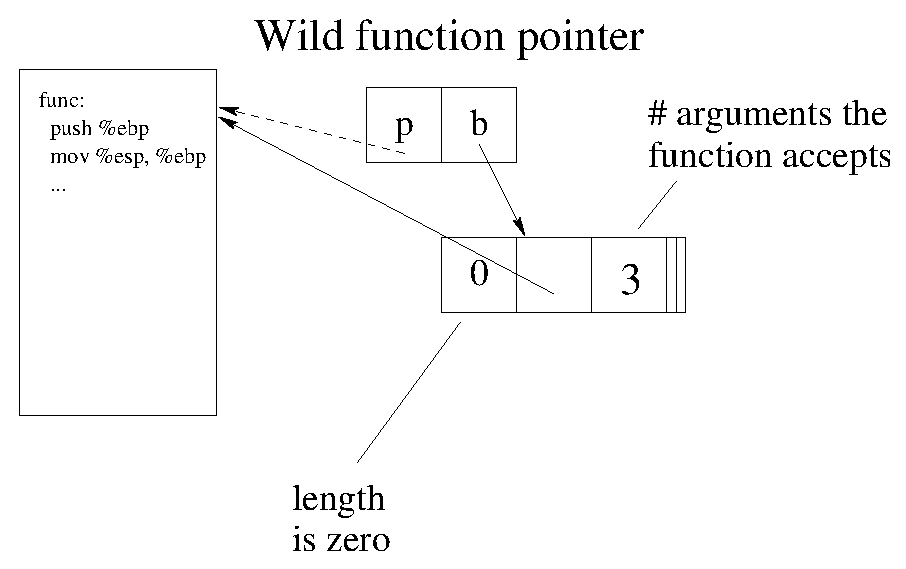
\includegraphics[scale=0.7]{wild_fn.eps}
\clearpage% page: 3

\end{document}
